\documentclass[superscriptaddress,twocolumn,aps,prd,10pt,nofootinbib,preprintnumbers]{revtex4-2}
\usepackage{amsmath}
\usepackage{amssymb}
\usepackage{graphicx}
\usepackage[colorlinks=true, pdfstartview=FitV, linkcolor=red, citecolor=blue, urlcolor=blue]{hyperref}
\usepackage[pgf]{adjustbox}
\usepackage[normalem]{ulem}
\usepackage{here}
\usepackage[english]{babel}
\usepackage{alltt}

%%%%%%%%%% Start TeXmacs macros
\newcommand{\assign}{:=}
\newcommand{\tmop}[1]{\ensuremath{\operatorname{#1}}}
\newcommand{\tmtextit}[1]{\text{{\itshape{#1}}}}
\newcommand{\tmverbatim}[1]{\text{{\ttfamily{#1}}}}
\newenvironment{tmcode}[1][]{\begin{alltt} }{\end{alltt}}
%%%%%%%%%% End TeXmacs macros

\begin{document}

\title{A Memory Efficient Optimizer with Momentum and Sign}

\author{Peng-xu Jiang}
\email{shuiruge@whu.edu.cn}

\begin{abstract}
  We propose a memory efficient optimization algorithm for deep learning that
  uses only the sign of momentum. This optimizer is as fast as Adam, but
  occupies half of the memory that Adam does. We also give an analysis of the
  effect of decay factor, which is the only hyper-parameter in our algorithm
  except for the learning rate. We validate the analysis on the fashion-MNIST
  dataset.
\end{abstract}

\maketitle

\section{Background}

\subsection{Gradient Descent Method}

For minimizing a smooth loss function $L : \mathbb{R}^n \rightarrow
\mathbb{R}$, standard gradient descent method computes the gradient of $L$,
and iterates along the negative direction of gradient so as to decrease $L$ at
each iteration. Explicitly, let $t \in \mathbb{N}$ denotes the step of
iteration, thus the model parameters $\theta$ at step $t + 1$ is given by (for
each component $\alpha$)
\begin{equation}
  \theta^{\alpha}_{t + 1} = \theta_t^{\alpha} - \eta \nabla^{\alpha} L
  (\theta_t), \label{equation:gradient descent method}
\end{equation}
where the $\eta$ is the learning rate. Since $L$ is smooth, we have $L
(\theta_{t + 1}) < L (\theta_t)$ as long as the learning rate is sufficiently
small and $\nabla L (\theta_t) \neq 0$. Thus, the iteration
(\ref{equation:gradient descent method}) always decrease $L$ until reaching
its (maybe local) minimum.

\subsection{Momentum}

Problems arise when applying gradient descent method directly to minimize the
loss function computed on mini-batch. Because we feed mini-batch (rather than
full-batch) to the model when we compute the loss function, denoted by $L$,
there must be randomness in it. What we really want to minimize is the
deterministic $\hat{L}$, the loss function computed on full-batch. So, we hope
that, iterated by the gradient descent method (\ref{equation:gradient descent
method}), the trajectory $(\theta_0, \theta_1, \ldots)$ generated by $\nabla
L$ (what we can compute) and the $(\hat{\theta}_0, \hat{\theta}_1, \ldots)$ by
$\nabla \hat{L}$ (what we expect to compute but cannot) share the same limit
$\theta_{\star}$, the real best-fit value. Only when $\nabla L$ is
sufficiently close to $\nabla \hat{L}$ can this be done, which indicates that
we have to reduce the randomness from the stochastic gradient $\nabla L$.

Another way of thinking about the stochastic gradient is from information
perspective. Let $\delta L (\theta) \assign L (\theta) - \hat{L} (\theta)$,
which collects the randomness caused by the mini-batch in $L$. Thus,
\begin{equation}
  \nabla L (\theta) = \nabla \hat{L} (\theta) + \nabla \delta L (\theta) .
  \label{equation:stochastic gradient}
\end{equation}
The information in the gradient $\nabla \hat{L} (\theta)$ is thus ``polluted''
by the noise $\nabla \delta L (\theta)$, making it hard for the model
parameters to find the correct directions to move.

An efficient method that reduces randomness is averaging. Let $\{ X_i |i = 1,
\ldots, n \}$ a set of i.i.d. random variables, each having variance
$\tmop{Var} [X]$. By central limit theorem, the variance of the averaged, $(1
/ n)  \sum_i X_i$, is decreased by a factor $1 / n$, thus becomes $\tmop{Var}
[X] / n$. In the same way, we can cache the most recent $n$ gradients $\{
\nabla L (\theta_{t - n + 1}), \ldots, \nabla L (\theta_t) \}$ at step $t$.
Then, average over the cache to get the gradient used for iteration, $(1 / n)
\sum_{i = t}^{t - n + 1} \nabla L (\theta_i)$. In this way, the variance of
randomness in $L$ is decreased by a factor $1 / n$. By adjusting the value of
$n$, the randomness can be limited sufficiently.

This ``bare'' average calls for caching the most recent gradients. It is very
memory intensive when the dimension of $\theta$ goes high. A smarter method is
moving average: given $\gamma \in (0, 1)$, the moving average of $\nabla L
(\theta_t)$, denoted by $g_t$, is computed by iteration (for each component
$\alpha$)
\begin{equation}
  g^{\alpha}_t = \gamma g^{\alpha}_{t - 1} + (1 - \gamma) \nabla^{\alpha} L
  (\theta_t), \label{equation:moving average}
\end{equation}
We initialize $g_t$ by zero vector, thus $g_0^{\alpha} = 0$. The $\gamma$,
called decay factor, determines how much old information from $g_{t - 1}$ is
to be ``forgotten'', and how much new information of from $\nabla L
(\theta_t)$ is to be ``memorized''. The $g_t$ can be seen as a weighted
average of $\{ \nabla L (\theta_0), \ldots, \nabla L (\theta_t) \}$, where the
recent gradients have greater weights and the remote have less. Then, we
iterate the $\theta_t$ by $g_t$ instead of $\nabla L (\theta_t)$, as
\begin{equation}
  \theta^{\alpha}_{t + 1} = \theta^{\alpha}_t - \eta g^{\alpha}_t .
  \label{equation:moving average 2}
\end{equation}


Moving average of gradient was first applied to gradient descent in
1986.\cite{backprop} Later, the
efficiency of moving average was usually explained as avoiding getting stucked
into local minima. They compared moving average of gradient to the momentum in
physics: the ``heavy ball'' rushes out of a local minimum with large
``momentum''. But, in a space with extremely high dimension, it is rare to
encounter a local minimum, but saddle points
instead.\cite{saddle} So, this
explanation cannot be faithful.

\subsection{Gradient Descent by the Sign of Gradient}

While training deep neural networks. it is often found that $\nabla^{\alpha} L
(\theta_t)$ varies greatly from component to component, for $\theta_t =
\theta_0, \ldots, \theta_{\star}$. This indicates that some components are too
inert to change (because their ratios are very small) while some are extremely
restless (because their ratios are very large). This non-synchronization slows
down the training process.

In 1992, Martin Riedmiller and Heinrich Braun proposed an algorithm called
\tmverbatim{rprop} (short for resilient back-propagation) that can release
this non-synchronization.\cite{rprop} It
uses the sign $\tmop{sign} (\nabla L (\theta_t))$ (rather than the gradient
$\nabla L (\theta_t)$ itself) in gradient descent iteration. In this way, all
components of gradient are ``standardized'' to be either $1$ or $- 1$ (rarely
being zero), thus become synchronized. The \tmverbatim{rprop} algorithm also
adaptively tunes the learning rate to make it more stable, which, however,
makes it impossible to deal with stochastic gradient.

Later in 2012, James Martens and Ilya Sutskever generalized the
\tmverbatim{rprop} algorithm to stochastic gradient. The new algorithm is
called \tmverbatim{rmsprop}.\footnote{Unpublished. We refer to
\href{https://www.cs.toronto.edu/~tijmen/csc321/slides/lecture\_slides\_lec6.pdf}{lecture
notes} by Geoffrey Hinton.} As it is named, it employs root mean square (RMS
for short) for approximating the sign of gradient, which helps stabilize the
stochastic gradient. Explicitly, it iterates a variable $s^{\alpha}_t$ (for
each component $\alpha$) with
\begin{equation}
  s_t^{\alpha} = \beta s_{t - 1}^{\alpha} + (1 - \beta)  (\nabla^{\alpha} L
  (\theta_t))^2, \label{equation:RMS}
\end{equation}
where $\beta \in (0, 1)$ and $s$ is initialized by zero vector, thus
$s_0^{\alpha} = 0$. This is another moving average with $\beta$ the decay
factor. Then, the iteration of gradient descent becomes (with $\epsilon$ a
tiny number for avoiding numerical error)
\begin{equation}
  \theta_{t + 1}^{\alpha} = \theta_t^{\alpha} - \eta \frac{\nabla^{\alpha} L
  (\theta_t)}{\sqrt{s^{\alpha}_t + \epsilon}} . \label{equation:RMS iteration}
\end{equation}
With moving average, the randomness is reduced; and the RMS
$\sqrt{s_t^{\alpha}}$ can be seen as an estimation of the $| \nabla \hat{L}
(\theta_t) |$, especially when $\eta$ is small and $\theta_t$ is slowly
varying. Thus, the last term in (\ref{equation:RMS iteration}) approximates
the $\eta \nabla L (\theta_t) / | \nabla \hat{L} (\theta_t) |$.

Finally, by combining \tmverbatim{rmsprop} and momentum, the state-of-the-art
optimization algorithm, named \tmverbatim{adam}, was proposed in
2014.\cite{adam} Explicitly, it first
computes momentum by equation (\ref{equation:moving average}). Then, it
computes the RMS by equation (\ref{equation:RMS}). And finally, iterates the
model parameters by (we omit the bias-correcting for simplicity)
\begin{equation}
  \theta^{\alpha}_{t + 1} = \theta^{\alpha}_t - \eta
  \frac{g_t^{\alpha}}{\sqrt{s^{\alpha}_t + \epsilon}} . \label{equation:Adam
  iteration}
\end{equation}
Again, by moving average, $g_t$ can be seen as an estimation of $\nabla
\hat{L} (\theta_t)$. Thus, the last term in (\ref{equation:Adam iteration})
approximates the $\eta \nabla \hat{L} (\theta_t) / | \nabla \hat{L} (\theta_t)
|$, which equals to $\eta \tmop{sign} (\nabla \hat{L} (\theta_t))$. This
motives us to consider using the $\eta \tmop{sign} (g_t)$ directly, since
$g_t$ has been an estimation of $\nabla \hat{L} (\theta_t)$ by moving average.

\section{Method}

\subsection{Gradient Descent by the Sign of Momentum}

Thus, we propose that, in the gradient descent iteration
(\ref{equation:gradient descent method}), we shall use the sign of momentum,
instead of the sign of gradient like \tmverbatim{rprop}, or of the gradient
rescaled by RMS like \tmverbatim{rmsprop}. That is, we shall use
\begin{equation}
  \theta_{t + 1}^{\alpha} = \theta_t^{\alpha} - \eta \tmop{sign}
  (g_t^{\alpha}) . \label{equation:RMS iteration}
\end{equation}
This is a \tmtextit{direct} combination of momentum (the strategy to reduce
the randomness in the gradient caused by mini-batch) and only using the sign
(the strategy employed in \tmverbatim{rprop} to force synchronizing the
gradients). In this way, there is no need to cache the term $s_t$ for RMS. The
memory occupation can be greatly decreased (to be half) comparing with
\tmverbatim{adam} algorithm.

As a summary, we implement our method using \tmverbatim{Numpy}.

{\small{\begin{tmcode}
def mas(loss_gradient,
        initial_theta,
        iteration_steps,
        learning_rate=2e-4,
        decay_factor=0.95):
    """Optimizer with Momentum and Sign (MaS)."""
    # Initialization:
    theta = initial_theta
    g = np.zeros(np.shape(theta))
    # Iteration:
    for t in range(iteration_steps):
        # Moving average
        g = (
            decay_factor * g +
            (1-decay_factor) * loss_gradient(theta)
        )
        # Iterate by sign of gradient
        theta = theta - learning_rate * np.sign(g)
    return theta
\end{tmcode}}}

\subsection{Effect of Decay Factor}

When $\gamma$ is close to $0$, the moving average $g_t$ is easy to forget the
old information of $\nabla L$. Indeed, the factor $\gamma \ll 1$ in
(\ref{equation:moving average}) implies $g_t \approx \nabla L (\theta_t)$,
thus no averaging at all. So, for make the moving average effective, $\gamma$
shall not be too small.

On the contrary, when $\gamma$ is close to $1$, the moving average $g_t$ is
hard to ``accept'' new information of $\nabla L$. Indeed, the factor $(1 -
\gamma) \ll 1$ in (\ref{equation:moving average}) implies $g_t \approx g_{t -
1}$. So, $g_t$ is hard to be modified when $\gamma$ is close to $1$. This is
equivalent to a large learning rate, leading to an ascent of loss function
instead of descent.

So, for efficiently and safely using moving average, the $\gamma$ shall be
moderate. And if, in practice, the randomness is so large that the moving
average can be effective only when $\gamma$ is close to $1$, then we shall
accordingly tune the learning rate $\eta$ to be smaller, so as to decrease the
loss function safely.

\section{Experiments and Results}

We make benchmark tests on fashion-MNIST dataset. We compare our method with
the state-of-the-art \tmverbatim{adam}, as well as many other optimization
algorithms such as \tmverbatim{adagrad}. The result can be found in figures
\ref{figure: benchmark test on ffd} and \ref{figure: benchmark test on
cnn}.\footnote{Code can be found in the repository:
\href{https://github.com/shuiruge/mas-optimizer}{https://github.com/shuiruge/mas-optimizer}.}
We use the same hyper-parameters (the default ones) throughout the tests.

\begin{figure}[h]
  \center{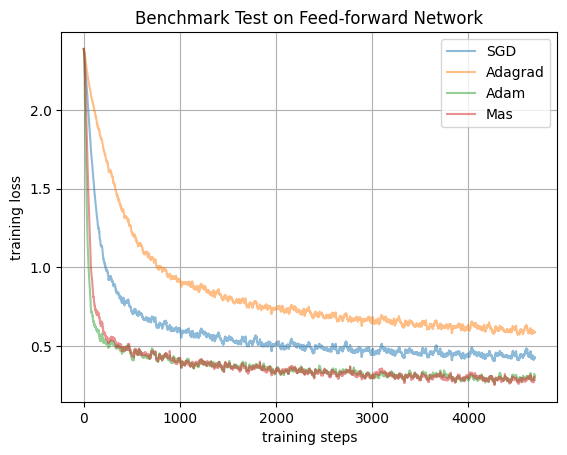
\includegraphics[width=6.97022169749443cm,height=5.22766627312082cm]{images/benchmark_test_on_ffd.png}}
  \caption{\label{figure: benchmark test on ffd}Comparing with other
  optimizers by training a feed-forward network on the training set of
  fashion-MNIST. Our method is denoted by ``Mas''. The feed-forward network
  contains two hidden layers, with $128$ and $64$ neurons respectively, and
  with ReLU activation. The output layer is linear. For hyper-parameters, we
  use the default values of each optimizer. The default learning rate of
  ``Mas'' is \tmverbatim{2E-4}; and the default decay factor is
  \tmverbatim{0.95}. For a better visualization, we smooth all the loss curves
  by moving average with decay factor $0.95$. It can be seen that our method
  is as fast as \tmverbatim{adam} (two curves overlap), and out-performs the
  rest.}
\end{figure}

\begin{figure}[h]
  \center{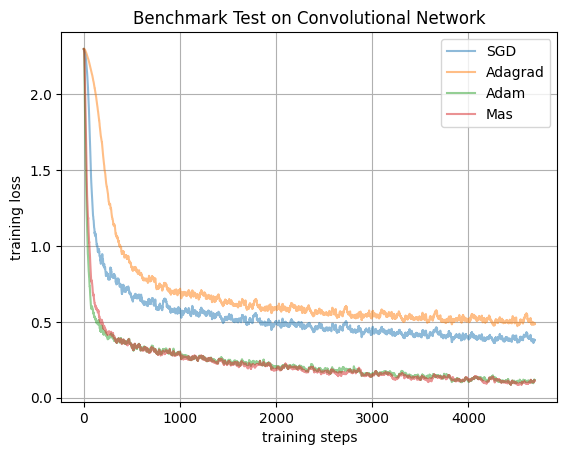
\includegraphics[width=6.97022169749443cm,height=5.22766627312082cm]{images/benchmark_test_on_cnn.png}}
  \caption{\label{figure: benchmark test on cnn}Comparing with other
  optimizers by training a convolutional network on the training set of
  fashion-MNIST. The convolutional contains layers in sequence:
  \tmverbatim{Conv2D(32, 3)}, \tmverbatim{ReLU()}, \tmverbatim{Conv2D(64, 3)},
  \tmverbatim{ReLU()}, \tmverbatim{MaxPool2D((2, 2))}, \tmverbatim{Flatten()},
  \tmverbatim{Dense(128)}, \ \tmverbatim{ReLU()}, and finally
  \tmverbatim{Dense(10)} as the output layer. Again, for hyper-parameters, we
  use the default values of each optimizer. And again, it can be seen that our
  method is as fast as \tmverbatim{adam} (the two curves overlap), and
  out-performs the rest.}
\end{figure}

It is found that our method is as fast as \tmverbatim{adam} algorithm. But
notice that we only cache $g_t$ as variable, while adam additionally caches
$s_t$, and that both $g_t$ and $s_t$ are vectors with the same dimension as
$\theta$, our method needs only half of the memory that \tmverbatim{adam}
occupies.

In the end, we also demonstrate the effect of decay factor $\gamma$ in
(\ref{equation:moving average}) in figure \ref{figure: decay factor}.

\begin{figure}[h]
  \center{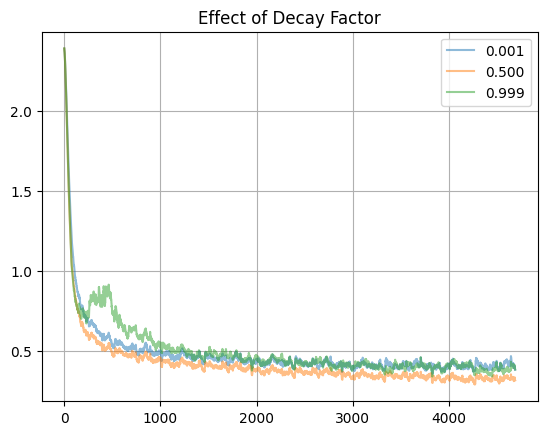
\includegraphics[width=6.97022169749443cm,height=5.22766627312082cm]{images/decay_factor.png}}
  \caption{\label{figure: decay factor}We demonstrate the effects of decay
  factors $0.001$, $0.5$, and $0.999$. The vertical axis represents for $L
  (\theta_t)$, and the horizontal axis for the $t$. The optimization is made
  on a feed-forward network with the same architecture as in figure
  \ref{figure: benchmark test on ffd}. We keep the learning rate default. It
  can be seen that a too small or too large decay rate (recall that decay rate
  is in $(0, 1)$) will slow down the optimization. Here, the best is the
  moderate (i.e. $0.5$, the yellow line). Notice the green curve (decay factor
  $0.999$) which jumps up in the period $t \in (0, 1000)$. This is consistent
  with our analysis that a large decay factor may cause an ascent of loss
  function.}
\end{figure}

\section{Conclusion and Discussion}

We have proposed a new algorithm that optimizes deep neural networks. From the
basic benchmark tests, we have found that our method is as fast as the
state-of-the-art \tmverbatim{adam}, but occupies only half of the memory that
\tmverbatim{adam} does. The key point is that there is no need to compute and
cache the RMS, and the sign of momentum is all you need.

Because of its efficiency in memory, as well as its state-of-the-art level
speed, it is a potential candidate for training large models.

\section{Acknowledgements}

We are grateful to Long Chen for his very useful discussions, to Jun Guo who
suggested to publish this method, and to Eden Li who supports me on every
aspects.

\bibliography{paper}
\bibliographystyle{plain}

\end{document}
